\section{Resource Control in Linux}

\mult{2}

\begin{concept}{Resource Competition}\\
    Operating systems must manage competition\\ for resources (res.):
    \begin{itemize}
        \item \textbf{Physical resources}: \\ Devices, bus systems, memory, etc.
        \item \textbf{Virtual resources}: Timers, locks, etc.
    \end{itemize}
    
    Resource control requires:
    \begin{itemize}
        \item Visibility: Knowing what resources are available
        \item Access control: Determine who can use res.
        \item Usage monitoring: Track resource consumption
        \item Unified approach: Coordinated res. management
    \end{itemize}
\end{concept}

\begin{definition}{Nice Process Concept}\\
    Traditional Unix approach to resource control:
    \begin{itemize}
        \item Users can be 'nice' by voluntarily releasing resources
        \item Modified by the \texttt{nice} command
        \item Limitations:
            \begin{itemize}
                \item No global definition, only relative values
                \item No strict and precise enforcement
                \item Users can only modify niceness of their own processes
                \item Limited applicability to specific resources
            \end{itemize}
    \end{itemize}
\end{definition}

\multend

\subsection{Linux Control Groups (cgroups)}

\mult{2}

\begin{definition}{Control Groups (cgroups)}
    Linux kernel feature for organizing tasks into hierarchical groups:
    \begin{itemize}
        \item Allows processes to be organized and \\ controlled collectively
        \item Strict enforcement of access and usage criteria
        \item Applies to sets of processes \& all future children
        \item Controls various types of resources \\ (CPU, memory, I/O, etc.)
    \end{itemize}
\end{definition}

\begin{theorem}{cgroups Terminology}
    Key concepts in cgroups:
    \begin{itemize}
        \item \textbf{cgroup}: Collection of processes\\ bound to limits/parameters
        \item \textbf{Subsystem} (Controller): \\Kernel component related to a resource type
        \item \textbf{Hierarchy}: \\ Arrangement of cgroups in a tree structure
        \item \textbf{Resource Controller}: \\ Implements behavior for specific resource type
    \end{itemize}
    
    Various controllers have been implemented:
    \begin{itemize}
        \item CPU controller: Limits CPU time
        \item Memory controller: Limits memory usage
        \item I/O controller: Controls disk I/O
        \item Network controller: Manages network bandwidth
        \item Devices controller: Controls device access
    \end{itemize}
\end{theorem}

\begin{definition}{cgroups Hierarchy}\\
    cgroups are organized in a hierarchical structure:
    \begin{itemize}
        \item Created by making subdirectories in the cgroup filesystem
        \item Limits defined at each level of the hierarchy
        \item Limits apply throughout the sub-hierarchy
        \item Descendant cgroups cannot exceed limits of ancestor cgroups
    \end{itemize}
\end{definition}

\begin{concept}{cgroups Implementation Approach}\\
    cgroups uses a filesystem-based approach:
    \begin{itemize}
        \item Communicates with Linux kernel via filesystem
        \item Virtual filesystem, stored in RAM
        \item Provides structured, standardized operations via I/O system calls
        \item Similar approach to /proc filesystem
        \item Implementation steps:
            \begin{itemize}
                \item Create tmpfs mount
                \item Create directory
                \item Mount resource control interfaces as files in directory
                \item Configure controls by editing files
                \item Associate processes (PIDs) with control configuration
            \end{itemize}
    \end{itemize}
\end{concept}



\multend

\subsubsection{cgroups Controllers}

\mult{2}

\begin{formula}{CPU Controller} manages CPU usage:
    \begin{itemize}
        \item Controls upper and lower limits of CPU shares
        \item Lower limit guarantees minimum CPU time when system is busy
        \item Upper limit restricts CPU time in each scheduling period
        \item Does not limit CPU usage if CPUs are not busy
    \end{itemize}
\end{formula}

\begin{formula}{Cpuset Controller} manages CPU assignment:
    \begin{itemize}
        \item Binds processes to specific CPUs
        \item Allows process isolation on multi-core systems
        \item Can be used to improve cache utilization
    \end{itemize}
\end{formula}

\begin{formula}{Memory Controller} manages memory usage:
    \begin{itemize}
        \item Reports and limits process memory, kernel memory, and swap usage
        \item Sets hard and soft limits on memory consumption
        \item Can enforce OOM (Out Of Memory) killing within cgroups
    \end{itemize}
\end{formula}

\begin{formula}{Blkio Controller} manages block device I/O:
    \begin{itemize}
        \item Limits access to block devices through throttling
        \item Sets upper I/O rate limits on devices
        \item Implements proportional-weight time-based division of disk I/O
        \item Can limit both read and write operations
    \end{itemize}
\end{formula}



\multend

\begin{example2}{CPU Controller Example}
    Limiting CPU usage for a group of processes:
    
\begin{lstlisting}[language=bash, style=basesmol]
# Create a cgroup for CPU control
mkdir /sys/fs/cgroup/cpu/limited_group
# Set maximum CPU usage to 10% (100ms in a 1000ms period)
echo 100000 > /sys/fs/cgroup/cpu/limited_group/cpu.cfs_period_us
echo 10000 > /sys/fs/cgroup/cpu/limited_group/cpu.cfs_quota_us
# Add a process to the cgroup
echo $PID > /sys/fs/cgroup/cpu/limited_group/cgroup.procs
# Run a CPU-intensive task and observe it being limited
# Even on an idle system, it won't exceed 10% of one CPU
\end{lstlisting}
\end{example2}

\begin{example2}{Device Controller Example}
    Restricting access to a device:
    
\begin{lstlisting}[language=bash, style=basesmol]
# Create a cgroup for device control
mkdir /sys/fs/cgroup/devices/group0
# By default, full permissions exist
cat /sys/fs/cgroup/devices/group0/devices.list
# Output: a *:* rwm (all devices, all permissions)

# Deny access to /dev/null (major 1, minor 3)
echo 'c 1:3 rwm' > /sys/fs/cgroup/devices/group0/devices.deny
# Add the current shell to the group
echo $$ > /sys/fs/cgroup/devices/group0/tasks
# Try to use /dev/null - it will fail
echo "test" > /dev/null
# Output: bash: /dev/null: Operation not permitted
\end{lstlisting}
\end{example2}

\subsection{cgroups Versions}

\begin{concept}{cgroups v1 vs v2}
    Linux has two implementations of cgroups:

    \begin{minipage}{0.3\linewidth}
        \textbf{cgroups v1}:
            \begin{itemize}
                \item Initial release in Linux 2.6.24
                \item Rapid adoption but \\ uncoordinated development
                \item Some inconsistencies between controllers
            \end{itemize}
        \end{minipage}
        \hspace{2mm}
        \begin{minipage}{0.65\linewidth}
        \textbf{cgroups v2}:
            \begin{itemize}
                \item Added in Linux 4.5
                \item Intended to replace v1 (but v1 continues to exist for compatibility)
                \item Currently implements a subset of v1 controllers
                \item Both versions can coexist, but a controller can't be used in both simultaneously
            \end{itemize}
    \end{minipage}
\end{concept}

\mult{2}

\begin{definition}{cgroups v1} two approaches to resource control:
    \begin{itemize}
        \item \textbf{Individual Resource Control}:
            \begin{itemize}
                \item Each controller mounted against a separate filesystem
                \item One controller associated with one hierarchy
            \end{itemize}
        \item \textbf{Collective Resource Control}:
            \begin{itemize}
                \item Multiple controllers co-mounted against a single filesystem
                \item Co-mounted controllers manage the same hierarchy
            \end{itemize}
    \end{itemize}
    
    Each cgroup is represented by a directory:
    \begin{itemize}
        \item Child cgroups represented as subdirectories
        \item Configuration files under each directory
        \item Files reflect resource limits and properties
    \end{itemize}
\end{definition}

\begin{definition}{cgroups v2}
    key differences from v1:
    \begin{itemize}
        \item All mounted controllers reside in a single unified hierarchy
        \item Simplified controller set
            \begin{itemize}
                \item io (replaces blkio)
                \item memory
                \item pids
                \item perf\_event
                \item rdma
                \item cpu
                \item freezer
            \end{itemize}
        \item Supports delegation (non-privileged users can manage subtrees)
        \item Supports thread mode (thread-level control)
    \end{itemize}
\end{definition}

\multend

\begin{concept}{Tasks vs Processes in cgroups v1}\\
    cgroups v1 distinguishes between tasks and processes:
    \begin{itemize}
        \item Process can consist of multiple threads (tasks)
        \item cgroups v1 allows independent manipulation of thread cgroup membership
        \item This can cause problems for controllers like memory (all threads share an address space)
        \item This ability has been limited in cgroups v2
    \end{itemize}
\end{concept}

\subsection{Working with cgroups}

\begin{KR}{Working with cgroups}
    \paragraph{Exploring cgroups}
    \begin{itemize}
        \item List available subsystems: \texttt{cat /proc/cgroups}
        \item View cgroup hierarchy: \texttt{tree /sys/fs/cgroup}
        \item Check cgroups created by systemd: \texttt{systemd-cgls}
        \item Monitor cgroup usage: \texttt{systemd-cgtop}
    \end{itemize}
    
    \paragraph{Creating and managing cgroups}
    \begin{itemize}
        \item Create a cgroup: \texttt{mkdir /sys/fs/cgroup/[controller]/[name]}
        \item Add process to cgroup: \texttt{echo [PID] > /sys/fs/cgroup/[controller]/[name]/cgroup.procs}
        \item Set CPU limit: \texttt{echo [value] > /sys/fs/cgroup/cpu/[name]/cpu.cfs\_quota\_us}
        \item Set memory limit: \texttt{echo [value] > /sys/fs/cgroup/memory/[name]/memory.limit\_in\_bytes}
        \item Remove cgroup: \texttt{rmdir /sys/fs/cgroup/[controller]/[name]}
    \end{itemize}
    
    \paragraph{Working with systemd cgroups}
    \begin{itemize}
        \item Create transient cgroup: \texttt{systemd-run --unit=[name] --slice=[slice] [command]}
        \item Set resource limits: \texttt{systemctl set-property [unit] [property]=[value]}
        \item Example: \texttt{systemctl set-property user.slice CPUQuota=20\%}
    \end{itemize}
\end{KR}

\begin{code}{Mounting cgroups v1}
    Mounting cgroups controllers:
    
\begin{lstlisting}[language=bash, style=basesmol]
# Create a tmpfs mount for cgroups
sudo mount -t tmpfs -o size=10M tmpfs /sys/fs/cgroup

# Mount a single controller (individual resource control)
sudo mount -t cgroup -o cpu none /sys/fs/cgroup/cpu

# Co-mount multiple controllers (collective resource control)
sudo mount -t cgroup -o cpu,cpuacct none /sys/fs/cgroup/cpu,cpuacct
\end{lstlisting}

    It's not possible to mount the same controller against multiple hierarchies.
\end{code}

\begin{code}{Creating and Managing cgroups v1}
    Basic cgroup management:
    
\begin{lstlisting}[language=bash, style=basesmol]
# Create a new cgroup
mkdir /sys/fs/cgroup/cpu/cg1

# Add the current process to the cgroup
echo $$ > /sys/fs/cgroup/cpu/cg1/cgroup.procs

# Add a specific process to the cgroup
echo <PID> > /sys/fs/cgroup/cpu/cg1/cgroup.procs

# Remove a cgroup (must be empty of processes and child cgroups)
rmdir /sys/fs/cgroup/cpu/cg1
\end{lstlisting}

    When adding a process to a cgroup, all threads in the process are moved together.
\end{code}

\begin{example2}{Using systemd Resource Control}
    Controlling resource limits with systemd:
    
\begin{lstlisting}[language=bash, style=basesmol]
# View current system slices
systemctl list-units --type=slice

# Check user slice settings
systemctl show user.slice

# Limit CPU usage for all user processes to 20%
sudo systemctl set-property user.slice CPUQuota=20%

# Create a resource-limited service
cat << EOF > /etc/systemd/system/limited-service.service
[Unit]
Description=Resource Limited Service

[Service]
ExecStart=/usr/bin/sha1sum /dev/zero
CPUQuota=10%
MemoryLimit=100M

[Install]
WantedBy=multi-user.target
EOF

# Reload systemd and start the service
sudo systemctl daemon-reload
sudo systemctl start limited-service

# Monitor resource usage
systemd-cgtop
\end{lstlisting}
\end{example2}

\begin{example2}{Creating a Custom CPU Control}
    Creating a CPU affinity control from scratch:
    
\begin{lstlisting}[language=bash, style=basesmol]
# Create a tmpfs mount
sudo mkdir -p /mnt/cgroups
sudo mount -t tmpfs none /mnt/cgroups

# Mount cpuset controller
sudo mkdir -p /mnt/cgroups/cpuset
sudo mount -t cgroup -o cpuset none /mnt/cgroups/cpuset

# Create a cgroup
sudo mkdir /mnt/cgroups/cpuset/group1

# Configure required memory settings first
echo 0 > /mnt/cgroups/cpuset/group1/cpuset.mems

# Restrict to CPUs 0 and 1 only (assuming 4 CPUs)
echo "0-1" > /mnt/cgroups/cpuset/group1/cpuset.cpus

# Run CPU-intensive processes
for i in {1..4}; do
  # Create processes
  sha1sum /dev/zero &
  # Get PID and add to cgroup
  PID=$!
  echo $PID > /mnt/cgroups/cpuset/group1/cgroup.procs
  echo "Added process $PID to CPU-restricted group"
done

# Check CPU assignment with taskset
for pid in $(cat /mnt/cgroups/cpuset/group1/cgroup.procs); do
  taskset -p $pid
done
\end{lstlisting}
\end{example2}

\begin{KR}{System Call Analysis}
    \paragraph{Key concepts}
    \begin{itemize}
        \item fork() duplicates current process
        \item exec() family replaces current process image
        \item Code after exec() only runs if exec() fails
        \item Count processes by tracing fork() calls
    \end{itemize}
    
    \paragraph{Analysis steps}
    \begin{itemize}
        \item Draw execution tree showing parent/child branches
        \item Mark where each printf() executes
        \item Identify exec() calls that replace process image
        \item Determine unreachable code after successful exec()
    \end{itemize}
\end{KR}

\begin{example2}{System Call Analysis}
    Analyze the output of a program using fork() and exec():
    
\begin{lstlisting}[language=C, style=basesmol]
int pid = fork();
printf("%s\n", "[1] Time for case distinction");
if (pid) {
    printf("%s\n", "[2] Starting emacs/fstab");
    execl("/bin/emacs", "/etc/fstab", (char *)NULL);
} else {
    printf("%s\n", "[3] Starting emacs/hosts");
    execl("/bin/emacs", "/etc/hosts", (char *)NULL);
}
printf("%s\n", "[4] Two editors started successfully");
// More code follows...
\end{lstlisting}
    
    \tcblower
    
    \textbf{Analysis:}\\
    Programm startet mit 2 Editoren:\\
    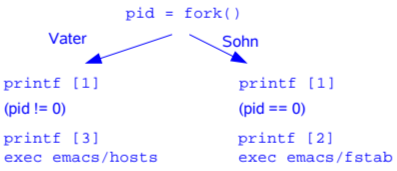
\includegraphics[width=0.5\linewidth]{system_calls_SEP07.png}

    \begin{itemize}
        \item Two editors are started
        \item Output: [1], [1], [2], [3]
        \item The code after execl() calls is never reached
        \item execl() replaces the process image, so [4] is never printed
    \end{itemize}
    
    \textbf{Execution flow:}
    \begin{itemize}
        \item fork() creates parent and child
        \item Both print [1]
        \item Parent (pid $\neq$ 0) prints [2], then execl() replaces it with emacs
        \item Child (pid == 0) prints [3], then execl() replaces it with emacs
    \end{itemize}
\end{example2}

